\documentclass[a4paper,10pt]{article}
\usepackage[utf8]{inputenc}
\usepackage[T1]{fontenc}
\usepackage[french]{babel}
\usepackage[normalem]{ulem}
\usepackage{geometry}
\usepackage{lmodern}
\usepackage{graphicx}
% \usepackage{setspace}
% \usepackage{titlesec}
\usepackage{geometry}
\usepackage{placeins}
% \usepackage{epsfig}
% \usepackage{hyperref}
% \usepackage{url}
% \usepackage{cite}
% \usepackage{listings}
% \usepackage{xcolor}


%\lstset{
%language=Java,
%basicstyle=\normalsize,
%upquote=true,
%aboveskip={1.5\baselineskip},
%columns=fullflexible,
%showstringspaces=false,
%extendedchars=true,
%breaklines=true,
%showtabs=false,
%showspaces=false,
%showstringspaces=false,
%identifierstyle=\ttfamily,
%keywordstyle=\color[rgb]{0,0,1},
%commentstyle=\color[rgb]{0.133,0.545,0.133},
%stringstyle=\color[rgb]{0.627,0.126,0.941},
%}

\geometry{top=3cm, bottom=3cm, left=2cm, right=2cm}

\title{Rapport\\Architecture Logicielle\\Jeu 2D autour d'un framework\\Année 2015/2016 }
\author{Raphaël Jorel, Antoine Laulan}



\begin{document}


\begin{figure}
    \begin{center}
    
\includegraphics[scale=0.7]{images/logo-bdx.pdf}
    \end{center}
\end{figure}
\maketitle

\newpage
% \tableofcontents
% \newpage



\newpage
\section{Introduction }
Notre jeu a été produit dans le cadre de l'UE architecture logicielle. Le but étant de créer un jeu à l'aide
d'un framework fourni et cela sans modifier celui-ci.
Dans ce rapport nous présenterons notre jeu et nous fournirons une critique du \textit{framework} utilisé. \\

Comme le sujet était libre, nous avons choisi de recréer une copie simplifiée du célèbre jeu Breakout.
Simple en apparence, mais qui nous aura quand meme donner du fil à retordre sur certains problèmes
que nous ne soupcionnions pas. Nous en parlerons d'ailleurs dans une partie dédiée.
%A voir si on laisse une intro, mais je trouve bizarre de pas en mettre en fait

\section{Firewall Breaker}
\subsection{Présentation}
    Tout d'abord, une petite image pour apprécier le rendu du jeu et des \textit{assets} qui ont été
    utilisés (tirée d'un Mac, tellement plus joli) :

\FloatBarrier
		\begin{figure}[!h]
    		\begin{center}
	   	  	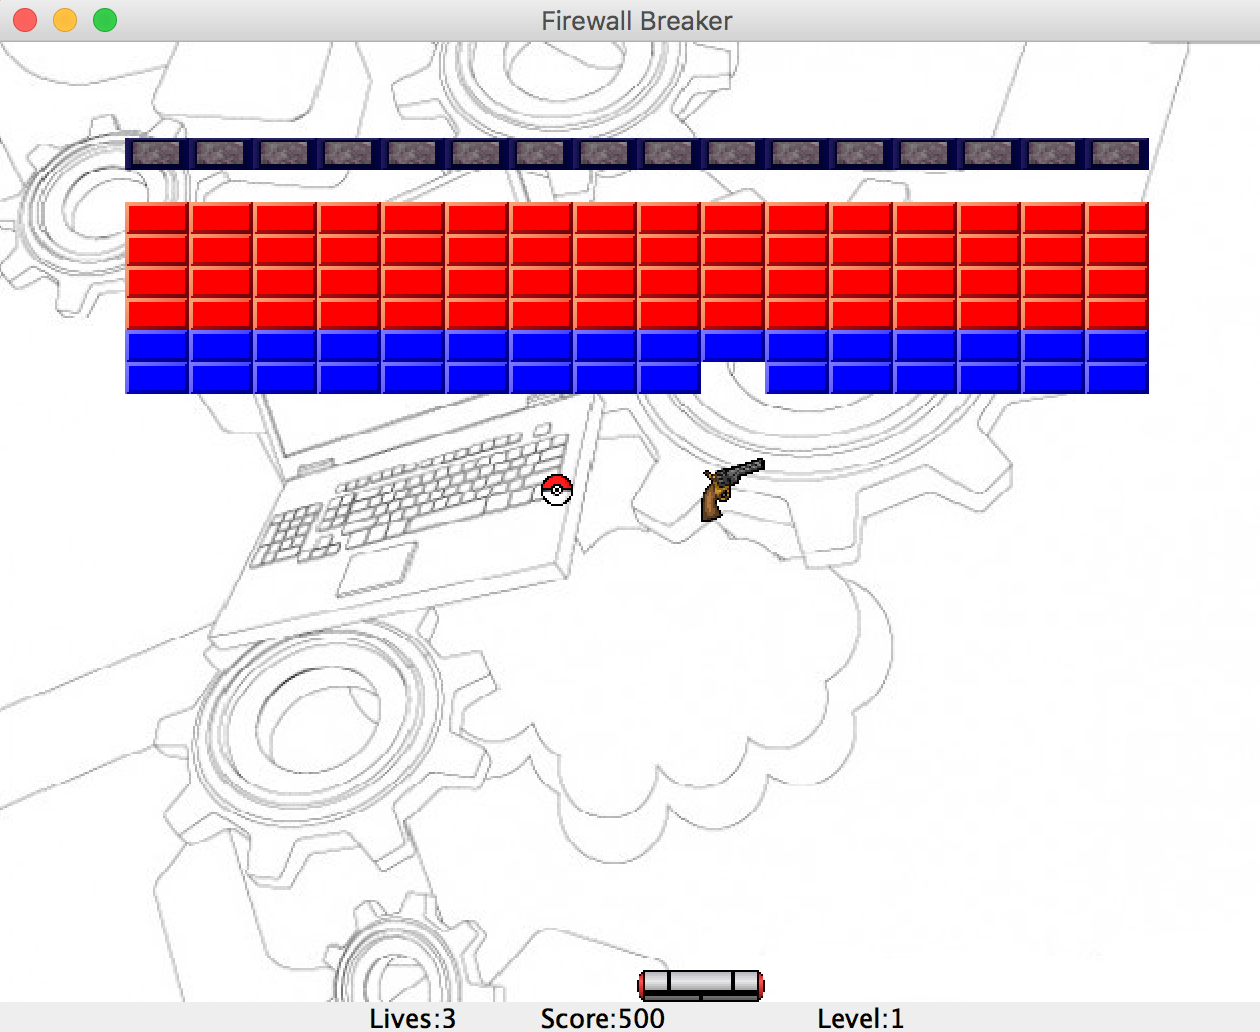
\includegraphics[scale= 0.5]{images/gameView.png}
          	\caption{Vue du jeu}
    		\end{center}
		\end{figure}
\FloatBarrier

% Notre jeu est basé sur le principe d'un wall breaker.
Le joueur contrôle une palette et doit, en faisant rebondir la balle, détruire les briques pour gagner.
Pour se faire il peut être aidé de divers bonus et briques spéciales. La partie s'arrête lorsque le joueur
a détruit toutes les briques qui peuvent l'être, ou lorsque celui-ci n'a plus de vie.

\subsection{Fonctionnalités du jeu}
    \subsubsection{Le joueur}
        Le joueur ne peut faire que deux choses : aller à droite ou à gauche. Il doit rattraper la balle
        qui se déplace pour la relancer dans le jeu et ainsi casser les briques. Comme sus-dit, il pourra
        etre aider par différents bonus, et ainsi augmenter sa capacité de destruction.

    \subsubsection{La balle}
        La balle se déplace et rebondit sur les briques, les murs (invisibles sur les côtés) et le joueur.
        Ses rebonds gardent les memes angles lorsqu'elle rebondit sur les murs et les briques, mais suivant
        l'endroit où elle touche le joueur, elle gagne ou perd en vitesse.

    \subsubsection{Les briques}
        Il y a 4 sortes de briques :
        \begin{itemize}
            \item les basiques : elles n'ont aucun effet, à part rapporter des points,
            \item les incassables : elles font barrage à la balle et ne peuvent etre détruites,
            \item les briques de bonus : donc celle qui déclenche l'apparition aléatoire de bonus,
            \item les briques explosives : celles-ci explosent et cassent toutes les briques alentour
                    dans un rayon aléatoire.
        \end{itemize}

        Lorsque toutes les briques sont cassées, le niveau est terminé. Toutes les briques cassables
        ne nécessitent qu'un seul coup pour etre détruites.

    \subsubsection{Les bonus}
        Afin de varier un peu le jeu, les bonus sont relativement nécessaires. Nous avons mis
        \begin{itemize}
            \item des bonus de vie, classique, mais toujours aussi utile.
            \item la possibilité de tirer des salves de balles,
            \item des bombes, qui font exploser aléatoirement une briques, cassant évidemment
                    toutes celles qui se trouvent autour,
            \item le changement de la balle en balle enflammée (\textit{fireball}) qui ne rebondit
                    alors plus sur les briques mais passe à travers tout (sauf les briques incassables).
        \end{itemize}

        Chacun de ces bonus sont associés à des probabilités, ainsi le bonus de vie a moins
        de chance d'apparaître que les autres, car le nombre de vies est un élément cruxial à prendre
        en compte, et que nous ne souhaitons pas que le jeu soit trop facile.

    \subsubsection{La gestion des parties}
        Il est toujours agréable de pouvoir recommencer une partie, sans etre obligé de relancer un
        programme. Pour cela, la fonctionnalité \textit{new (game)} a été apportée, en plus de la
        possibilité de quitter. Par contre, il est impossible de suspendre une partie et de la reprendre,
        donc il faut que vous soyez vraiment sûr de n'avoir rien besoin de faire pendant vos parties
        (que l'on espérera enflammée, évidemment).


\subsection{Architecture}
    Un bon projet, c'est aussi une bonne architecture...
	Nous allons dans cette partie vous présenter l'architecture logicielle de notre jeu. Ceci sera fait à l'aide de
	diagrammes de classes.
	Nous metrons en évidence les connexions entre nos classes et les classes du framework.

% A voir si on met un diag de paquetage ou pas

	\subsubsection{Diagrammes de classe}

		\FloatBarrier
		\begin{figure}[!h]
    		\begin{center}
	  	  	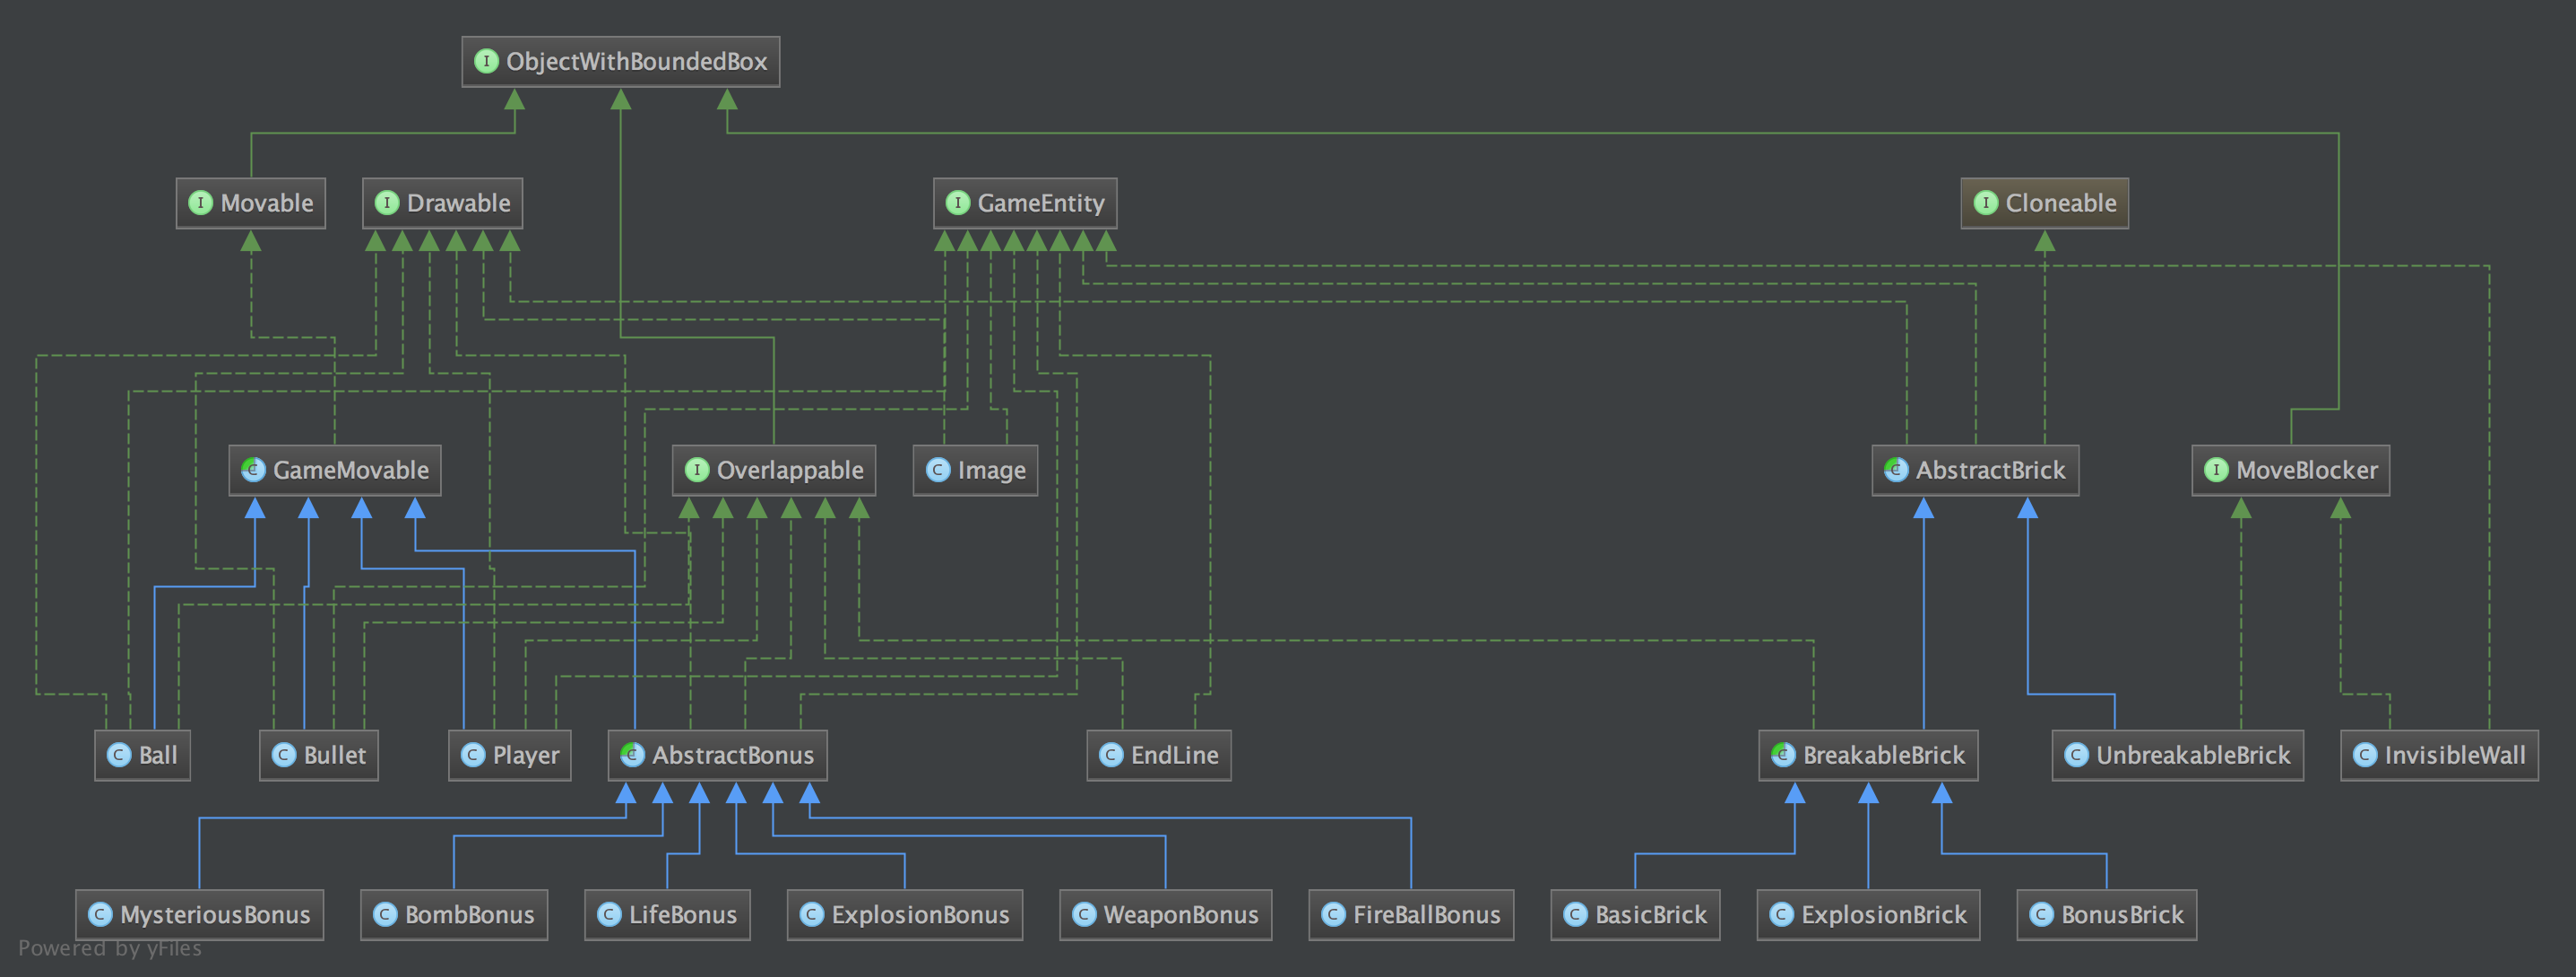
\includegraphics[scale=0.175]{images/entitiesDiag.png}
          	\caption{Diagramme de classe des entités}
    		\end{center}
		\end{figure}
		\FloatBarrier
		\paragraph{Description :}
		Voici le diagramme de classe regroupant les différentes entités de note jeu. \\

		% pour l'instant c'est dégeu mais c'est temporaire c'est juste histoire de poser le concept de couleur
		% car plusieurs classes sont relations donc j'ai regroupé tout dans un diag que on va différencier par les couleurs
% 		\FloatBarrier
% 		\begin{figure}[!h]
%     		\begin{center}
% 	  	  	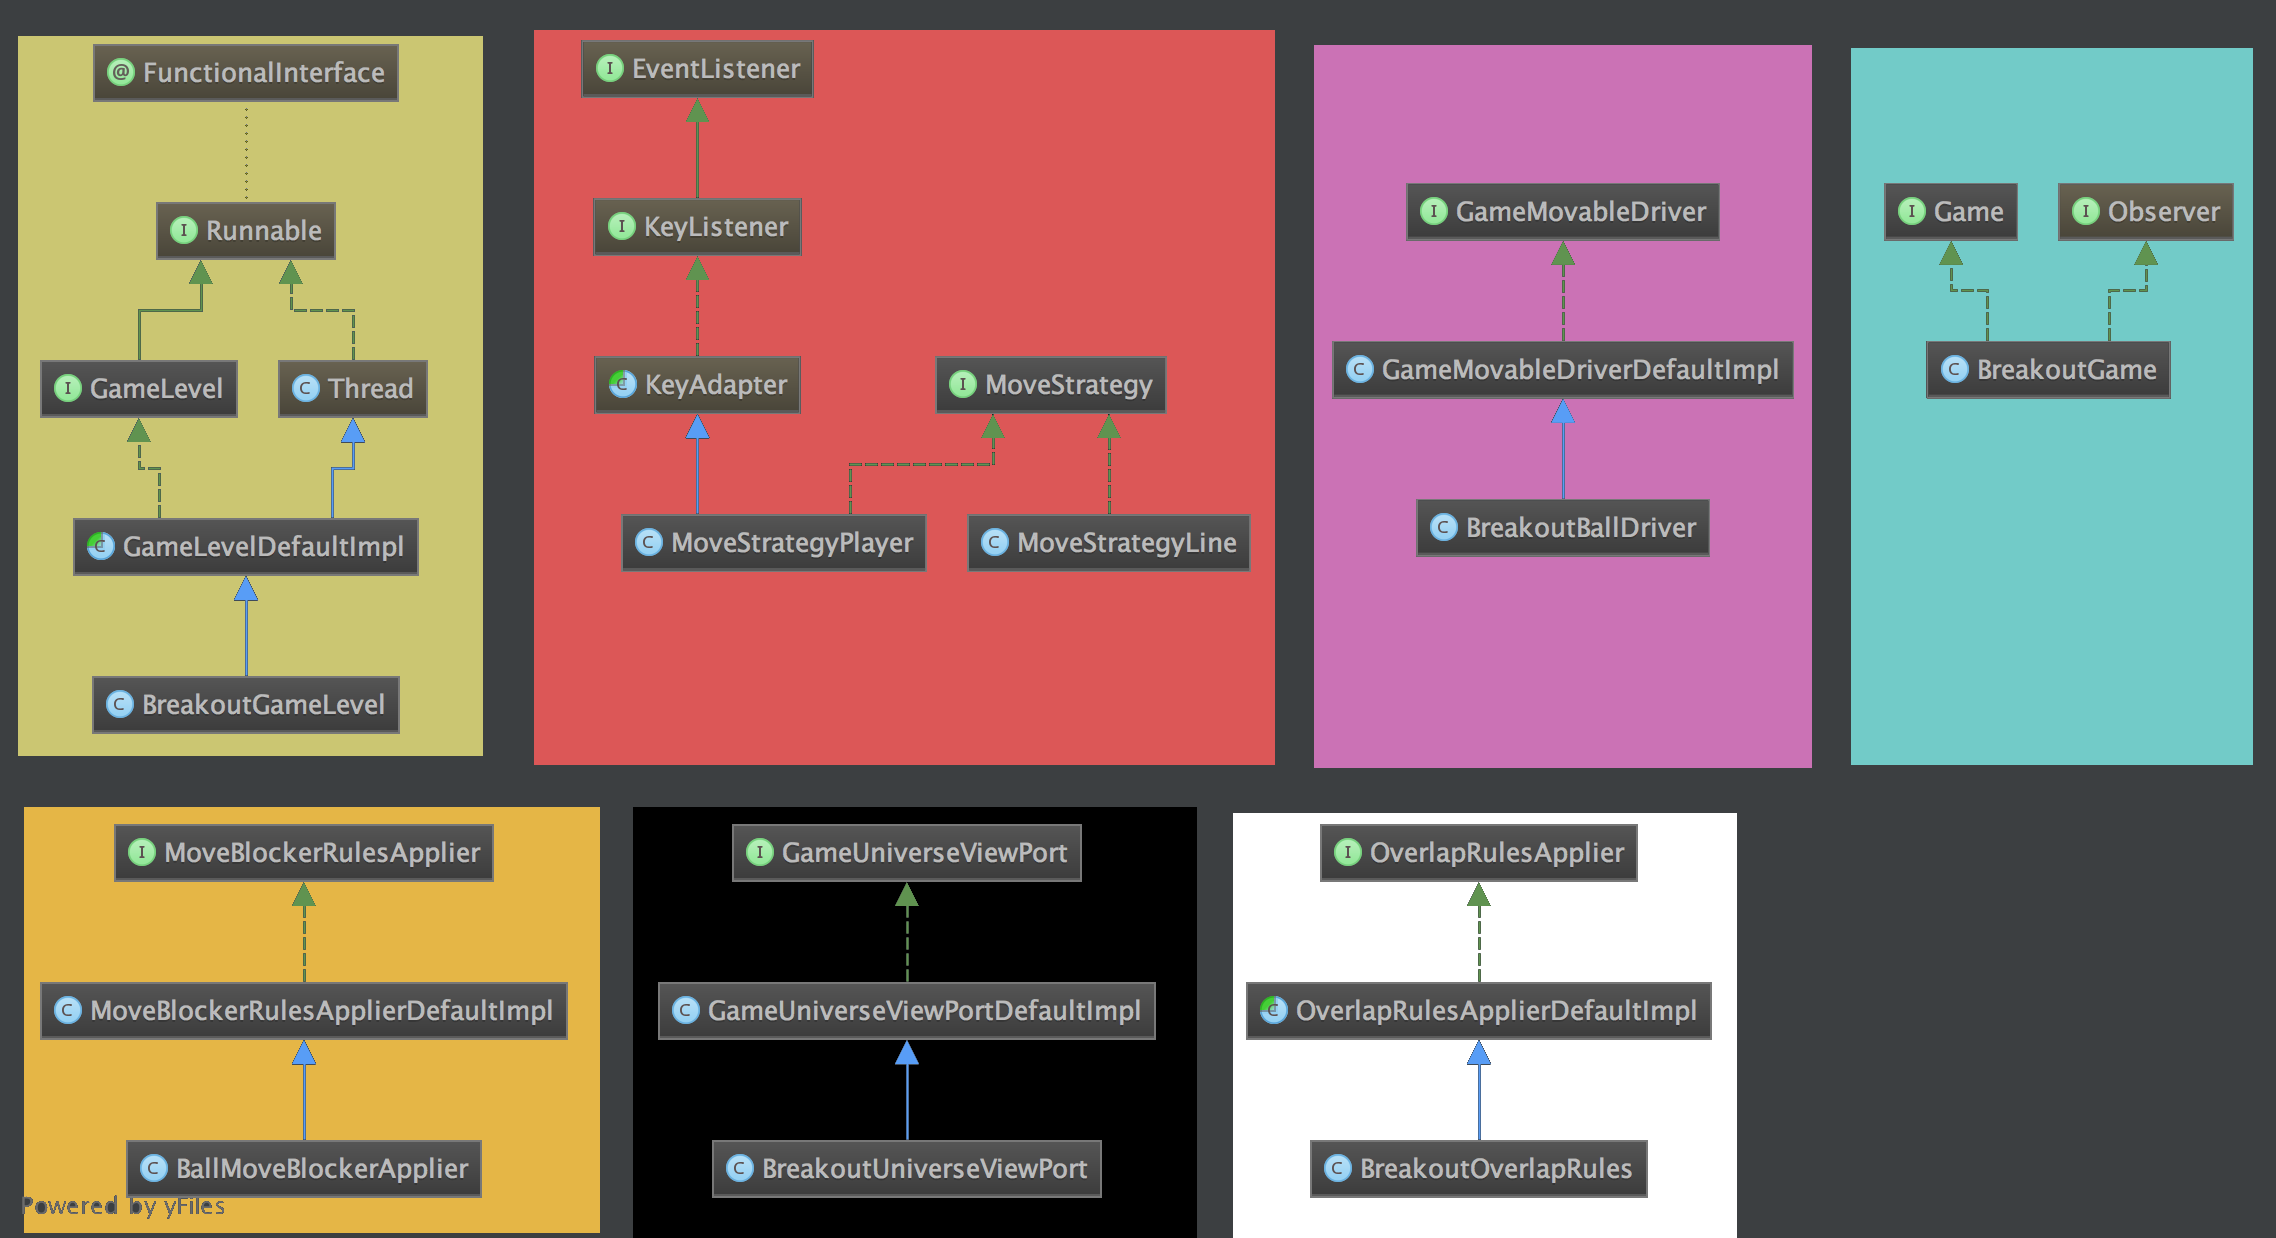
\includegraphics[scale=0.2]{images/severalDiagrams.png}
%           	\caption{Multi diagramme de classe}
%     		\end{center}
% 		\end{figure}
% 		\FloatBarrier
% 		\paragraph{Description :}
% 		Plusieurs classes forment de petits diagrammes de classes. Nous les avons regroupés dans une seule est même image. Pour les différencier
% 		nous avons utilisé un code couleur. Ce code couleur est détaillé dans la liste suivante : \\
% 		\begin{itemize}
% 		\item Diagramme jaune :
% 		\item Diagramme rouge :
% 		\item Diagramme violet :
% 		\item Diagramme bleu :
% 		\item Diagramme orange :
% 		\item Diagramme noir :
% 		\item Diagramme blanc :
% 		\end{itemize}


\subsection{Implémentations}
    Après cette présentation des possibilités offertes par le jeu et son architecture, parlons maintenant
    de l'implémentation du jeu, donc du travail qui a été effectué.

    \subsubsection{Les niveaux}
        Afin de ne pas avoir à écrire statiquement la configuration des briques d'un niveau, nous avons
        utilisé des fichiers externes pour le faire. Chaque type de brique est représentée par un numéro.
        Théoriquement, il est d'avoir un nombre de brique en largeur et en hauteur aussi grand qu'on le souhaite,
        il faut juste préciser cela dans le fichier de description, mais pour des raisons de jouabilité, il
        esr recommandé de se limiter à des grilles de 16x16. Ainsi, la balle a toujours la place de bouger. \\

        Pour éviter d'instancier les briques à chaque fois, nous nous sommes servis du \textit{design pattern prototype},
        cela permettant d'avoir les briques de bases dans un tableau et ensuite de les cloner en fonction du
        fichier de description.

    \subsubsection{Les stratégies de déplacement}
        Les stratégies permettent de définir comment un objet va se déplacer. Pour notre jeu, nous avons eu besoin
        de deux stratégies seulement : celle du joueur et celle des autres entités. Les autres entités
        se déplacent toujours en ligne droite, alors que le joueur bougent suivant l'action de l'utilisateur, et donc
        de la frappe du clavier.

    \subsubsection{La fenetre de jeu}
        En s'inspirant de l'exemple d'utilisateur du \textit{framework}, nous avons créé une fenetre de jeu semblable,
        mais évidemment plus appropriée au jeu de Breakout. La possibilité de recommencer une partie et de la quitter
        font partie des deux seules fonctionnalités de la fenetre d'affichage. \\

        Afin de gérer la fonction \textit{new}, nous avons remanié l'exemple donné pour lui permettre de fonctionner
        correctement. Nous gérons les niveaux dans une file de \textit{threads} qui attendent d'etre lancé. Lorsque la file
        est vide, le jeu se bloque et attend. Une fois que le joueur a fait \textit{new}, la file de \textit{threads} est
        à nouveau remplie, et ces derniers peuvent etre relancer. Si jamais l'utilisateur fait \textit{new} avant
        la fin du jeu, le \textit{thread} courant est arreté, pour pouvoir repartir sur un jeu ``neuf''.

    \subsubsection{Les rebonds}
        Une mauvaise impression sur les rebonds peut rebuter quelque peu l'utilisateur. Nous ne pensions pas que
        cette partie serait la plus compliquée, mais c'en était pas loin. Nous effectuons les rebonds de façon
        séparées sur les briques cassables et incassables, car ces dernière sont considérées comme \textit{blockers}.
        Lorsque la balle est bloquée par l'une d'elle, nous proposons au \textit{driver} de la balle des possibilités
        de stratégies à essayer afin de choisir celle qui est applicable, pour que la balle puisse continuer à bouger. \\
        Par contre, lorsqu'elle entre en collision avec les autres, c'est différent.
%         Et là, faut expliquer.

        En ce qui concerne les murs, nous ne faisons qu'inverser la vitesse sur l'axe des ordonnées ou des abscisses suivant
        que le mur est horizontale ou non.

        \paragraph{Calcul du point de collision}
            Les murs et les briques incassables sont des \textit{blockers}, c'est-à-dire que le système calcule avant de
            déplacer les entités mobiles (comme la balle) si ces dernières rentrent en collision avec les \textit{blockers}.
            Et si c'est le cas, l'entité ne sera pas déplacée. Ceci pose un problème lorsque la balle est trop rapide. En
            effet, le système considérera qu'une entité ne pourra etre déplacée, alors qu'en raison de sa grande vitesse,
            elle ne sera pas collée à un mur ou une brique incassable. Pour rémédier au problème, il suffit de vérifier si
            la balle est effectivement collée ou pas, et ensuite calculer le point de collision si ce n'est pas le cas.
            Comme nous ne modifions la vitesse que sur l'axe des abscisses, ce calcul n'est pas effectué sur celui des
            ordonnées.

    \subsubsection{Gestion des briques}
        Les briques sont toutes issues de la meme classe abstraite. Cette classe gère quasiment tout, les briques ne font
        que définir des types qui seront utile pour identifier les entités qui se touchent. Principalement, elle
        précisent leur image qui sera affichée pour les identifier. \\

        Pour alléger la mémoire, bien que le jeu soit petit, il ne nous a pas paru logique que chaque briques aient
        son image, alors que beaucoup de briques ont les memes. Pour gagner de la place, nous avons utilisé un tableau
        statique dans la classe abstraite qui répertorie les images et qui ne rajoutent que celles qui ne sont pas
        encore chargée. Les briques se voient alors assigner un numéro d'image, qui correspond à l'indice dans le
        tableau.

    \subsubsection{Bonus}
        Les bonus n'ont pas été la partie la plus dur à implémenter et penser, bien qu'elle demanda un peu
        d'imagination. Le plus dur a finalement été de comprendre bien le \textit{framework} pour savoir
        comment arriver à nos fins.


\subsection{Limites du jeu}
Meme les grands jeux ont des limites, prenez par exemple \textit{Assassin's Creed Unity}... quoique dans ce cas,
il s'agisse plutôt de bugs. \\

La gestion des collisions n'a pas été chose simple, aussi il est assez remarquable par moment que la balle
ne rebondit pas comme souhaité. Cela vient principalement \textit{framework} qui permet difficilement d'avoir
conscience du contexte de la balle. De plus, ce dernier permet que la balle touche plusieurs briques à la fois,
ce qui peut entraîner des comportements inattendus, vu que la trajectoire de la balles sera modifiée plusieurs fois. \\

Pour des raisons qui nous échappe également, l'image des explosions ne disparaît pas certaines fois. Il est possible
que ce soit dû à des problèmes de collisions multiples d'une brique avec une bombe et une autre élément du jeu (les
balles tirées par exemple).

% Et puis merde quoi, si votre framework c'était pas de la merde comme ça, on aurait fait un truc bien !!!

% Cette partie sera utilisée pour expliquer quelles sont les limites du jeu. C'est à dire que nous expliquerons ce qui fonctionne mal ou ne fonctionne pas du tout.
% \begin{itemize}
% \item
% \item
% \item
% \end{itemize}

\subsection{Difficultés rencontrées}
Nous avons tout de même rencontrées plusieurs difficultés et nous en ferons la liste dans cette partie. Nous donnerons également "l'état" de cette difficulté dans la version actuelle du jeu.
% \begin{itemize}
% \item
% \item
% \item
% \end{itemize}


\section{Critiques du framework }
    Passons maintenant à une petite critique du \textit{framework}... il est toujours plus facile de critiquer que
    de faire, donc comme nous avons fait, place à la critique (bien méritée, vous en conviendrez).

    \paragraph{Nom des classes}
        Mention spéciale aux noms des classes fort longs parfois. Bien que cela explicite peut-etre le rôle
        de chaque classe, il est parfois bien compliqué de s'y retrouver, et de comprendre le fonctionnement,
        car les noms ne différent pas de beaucoup par moment. De plus, les suffixes \textit{DefaultImpl} alourdissent
        les noms et sont franchement inutile.

    \paragraph{Introspection}
        On nous a appris que l'introspection faisait perdre en performances. Et pourtant, le \textit{framework} s'en sert
        pour faire appel aux fonctions de gestion des collisions. Ceci permet d'ajouter que les règles de collision
        qui nous intéressent, mais n'oublions pas que les performances en patissent. De plus, cette technique est
        utilisée à deux endroit du code, et cela est appliqué à chaque itération du jeu.

    \paragraph{Image de fond}
        Pour créer un niveau, il est nécessaire d'avoir un \textit{viewport}, ce que le système fournit. Ce qui est
        par contre assez difficile à comprendre, c'est pourquoi la classe gérant \textit{viewport} par défaut
        comporte une méthode qui permet de modifier l'image de fond, alors que finalement la méthode récupérant
        cette image ne fait que renvoyer une chemin vers une image ? Et cela écrit en dur en plus ! Conclusion, une classe
        fille seulement pour une méthode qui fait un travail inattendu...

    \paragraph{Gestion des niveaux}
        Pourquoi avoir gérer les niveaux comme des threads ? Bonne question... une fois lancés, impossible de les
        relancer, impossible à cloner, gestion plus compliquée, etc... nous supposons que cela est pour permettre
        à l'\textit{EventDispatcher} de faire son travail avec l'interface du jeu, mais le travail pour gérer
        les niveaux est bien plus compliquée. \\
        D'ailleurs, l'exemple donné (le \textit{Pac Man}) ne gère pas du
        tout bien cela. Il suffit de rajouter un niveau au jeu pour se rendre compte que faire \textit{new} lance
        deux niveaux en meme temps. Mais cela vient d'une boucle \textit{foreach} sur les \textit{threads} et donc
        la liste de niveau de retrouve parcouru à deux endroits différents. De plus, le \textit{Pac Man} ne gère
        pas le \textit{new} lorsque le jeu est terminé. Et ceci est normal, car un \textit{thread} ne peut etre
        relancer. Pour pallier au problème, nous ne donnons que les chemins vers les fichiers de définition des
        niveaux et nous recréons des \textit{threads} à chaque \textit{new}. Si les \textit{threads} étaient
        clonable, cela aurait pu etre éviter...

    \paragraph{La facilité a un coût}
        Le \textit{framework} permet une mise en place rapide de jeux, et fournit les éléments nécessaires pour
        que cela soit jouable. Mais cette facilité est compensée par le fait qu'il n'est pas évident (à moins
        de réécrire certaines classes) de faire des choses très poussée. En effet, comme évoquée dans la partie
        implétementation, le système considère les collisions avec les \textit{blockers} de façon très basique
        en fait. Il n'y pas de vérifications qui permettrait d'approcher les \textit{blockers} de façon plus
        naturelle. C'est d'ailleurs pour cela que nous avons dû calculer nous-meme le point d'impact quand cela
        était nécessaire.

    \paragraph{Une classe de collision à rallonge}
        Loin de l'idée que les classes doivent etre courte pour etre plus facilement réutilisable, il y a peut-etre
        des limites. Autant pour la classe gérant la fenetre d'affichage, cela parait logique car il y a beaucoup
        de code pour mettre en place les éléments, autant des fois c'est évitable. Nous exposons ici la classe
        qui gére les collisions entre entités \textit{overlappable}. La côté pratique, c'est que tout est au
        meme endroit, celui qui l'est moins, c'est qu'avec quelques centaines de lignes de codes et des fonctions
        qui se nomment toutes \textit{overlapRule}, il n'est pas si évident de s'y retrouver.


\section{Conclusion}
    En guise de conclusion, nous dirons que le projet a été tout de meme fort agréable, bien que la compréhension
    du \textit{framework} ne fut pas triviale, et a été notre principal frein.  \\
    Ceci dit, faire un jeu
    a vraiment été agréable, de par de son côté evidemment ludique... et ça change de faire des sites web.
%     En gros, c'est de la grosse merde ce \textit{framework}... allez vous pendre, vous faites que de la merde.

\end{document}
\grid
